\chapter{Voltage Level Test}\label{app:VoltageLevelTest} 
\textbf{Name: Group 733}\\
\textbf{Date: 24/10 - 2016}

\subsubsection{Purpose}
Finding the influence of the battery voltage level in the final motor velocity applied by the motor speed controller. The quadcopter controller will account for this influence when setting the speed reference.

\subsubsection{Setup}
%\begin{figure}[H]
%	\centering
%	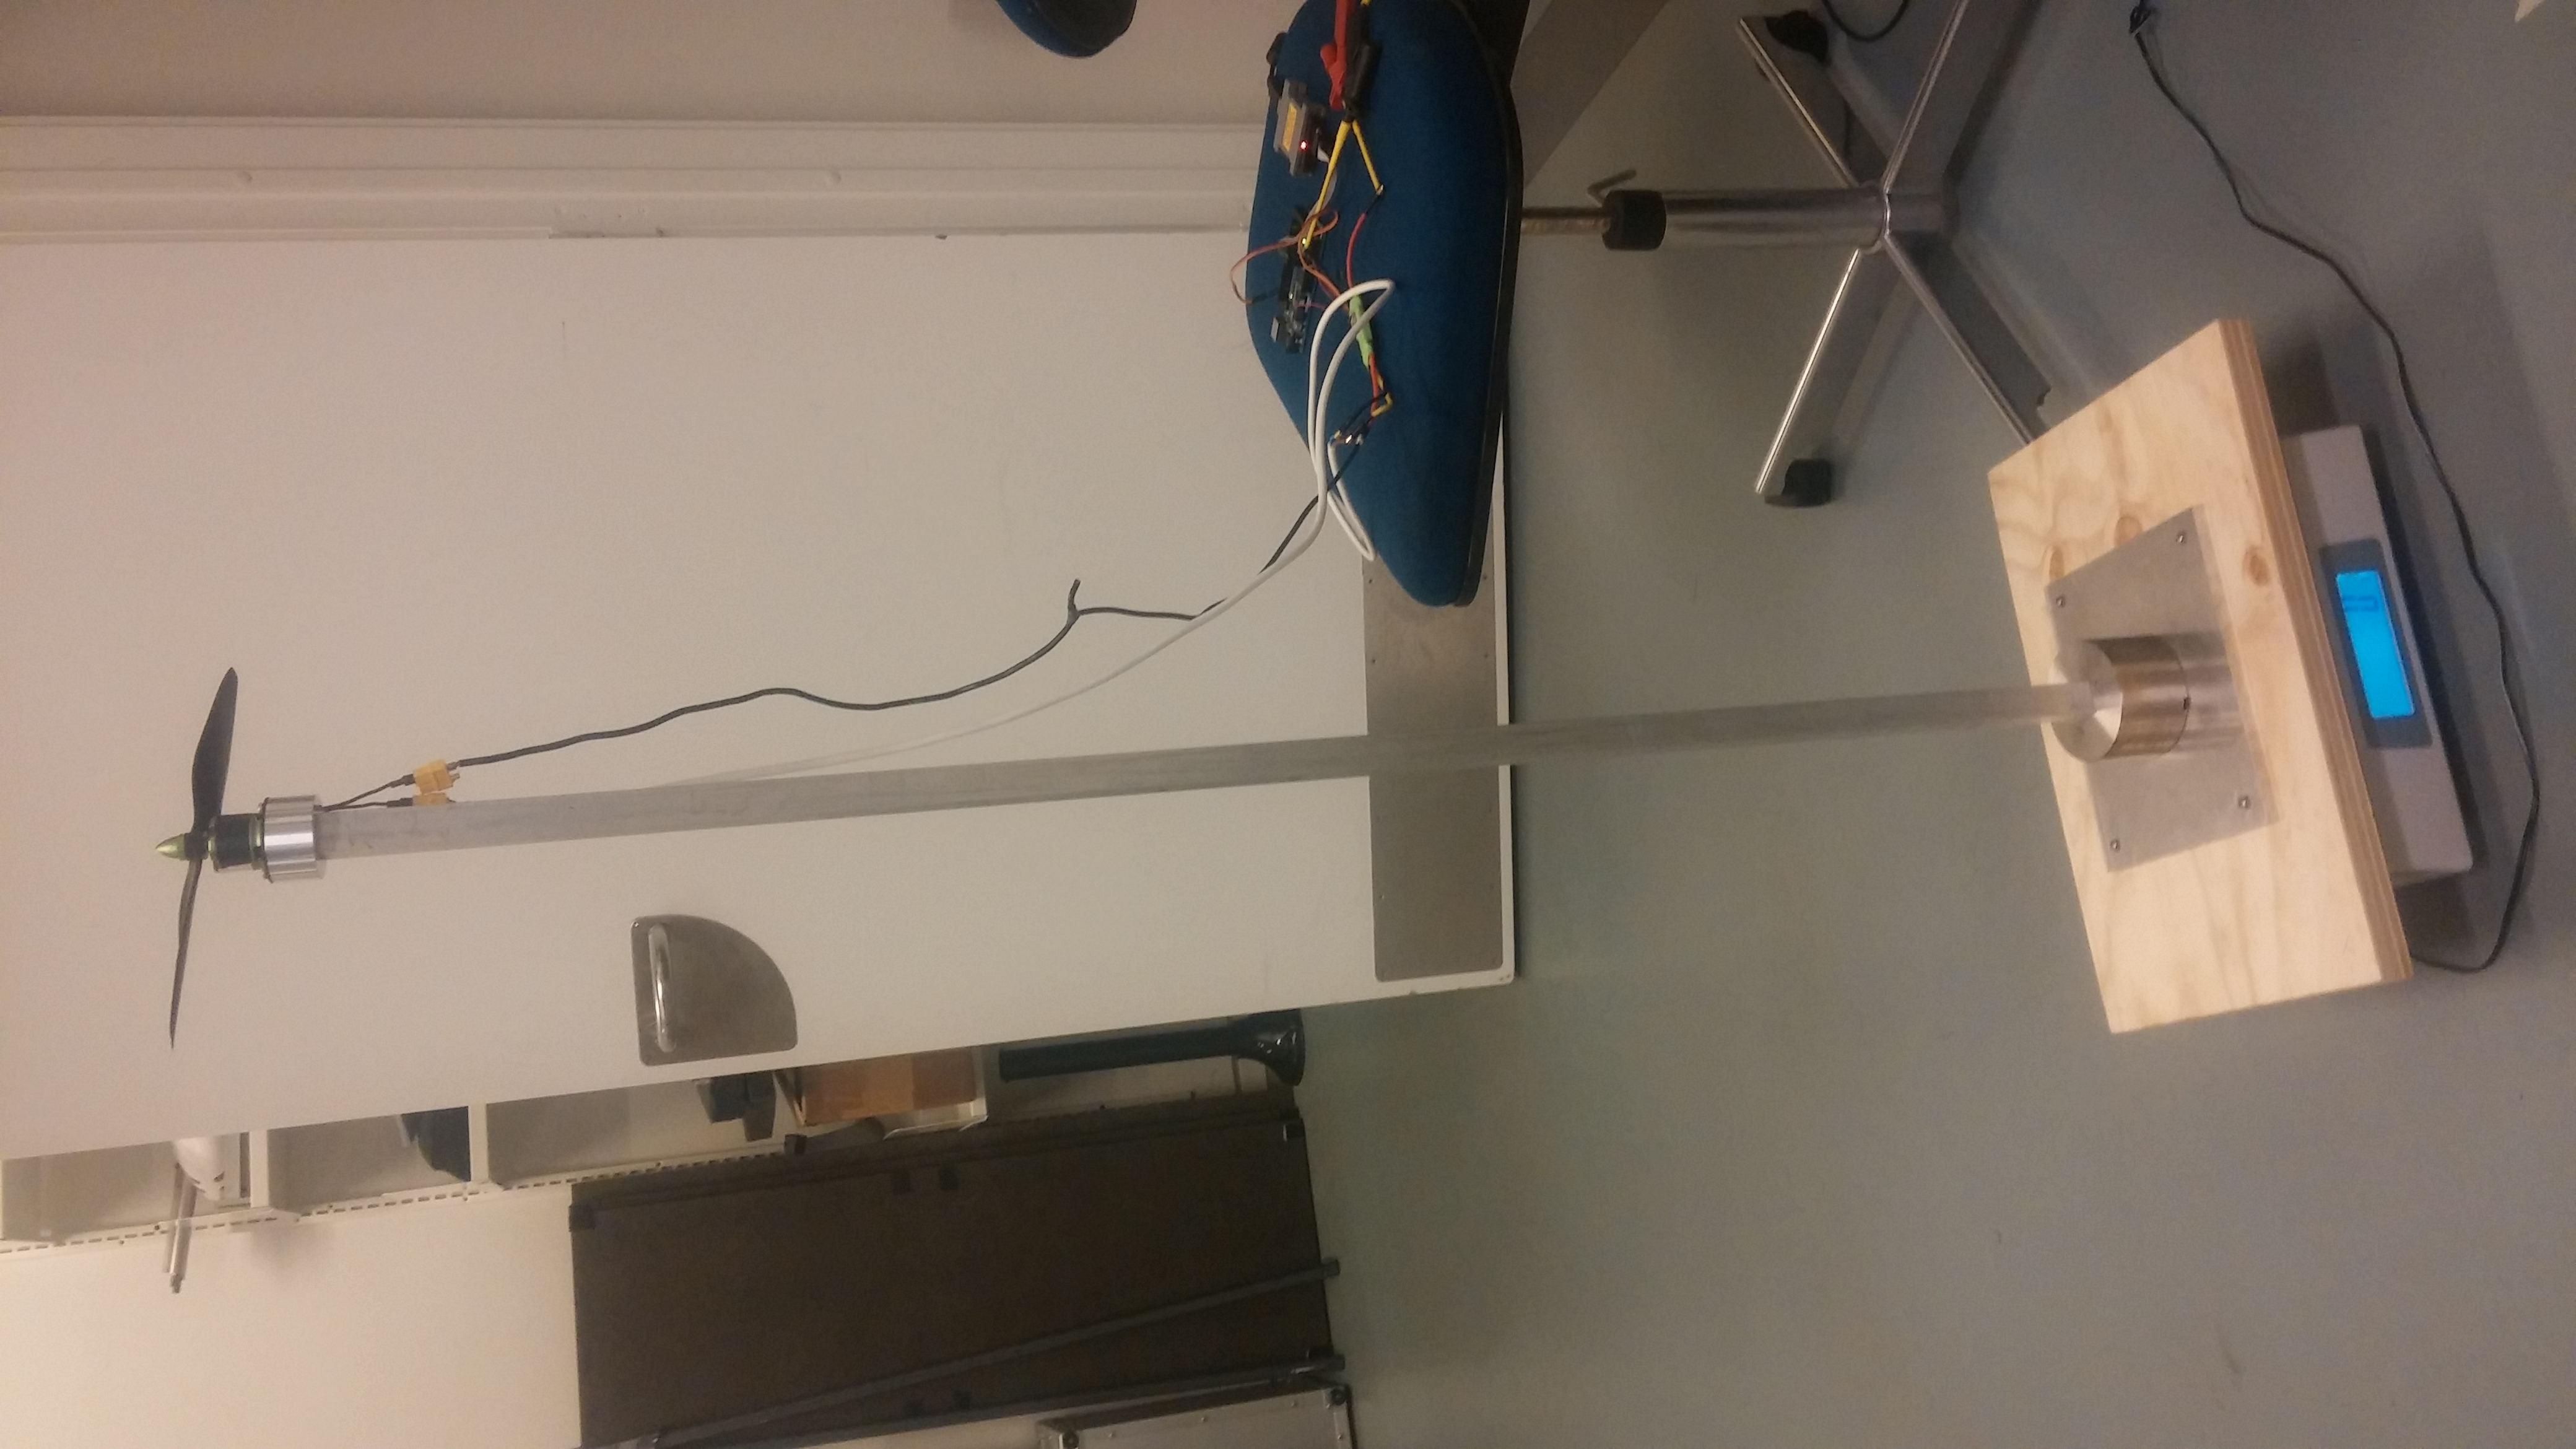
\includegraphics[scale=0.05,angle =-90]{figures/ThrustTestSetup}
%	\caption{The setup for the thrust test.}
%	\label{ThrustTest}
%\end{figure}

\subsubsection{List of Equipment}
\begin{table}[H]
	\begin{tabular}{|l|l|p{4.3cm}|}
		\hline%------------------------------------------------------------------------------------------------------------
		\textbf{Instrument}                          &  \textbf{AAU-no.}  &  \textbf{Type}                       \\
		\hline%------------------------------------------------------------------------------------------------------------
		Tachometer                                   &  08246             &  Shimpo DT-205		                   \\
		\hline%------------------------------------------------------------------------------------------------------------
	    Power Supply (11.1 V)                        &  64565             &  ES 030-5                 \\
		\hline%------------------------------------------------------------------------------------------------------------
		Processing Unit                              &  N/A               & Arduino Mega     \\
		\hline%------------------------------------------------------------------------------------------------------------
		Motor                                        &  N/A               & Multistar 2213-935     \\
		\hline%------------------------------------------------------------------------------------------------------------
		Motor Speed Controller                       &  N/A               &  -      \\
		\hline%------------------------------------------------------------------------------------------------------------
		Propeller                                    &  N/A               & Turnigy 1045R     \\
		\hline%------------------------------------------------------------------------------------------------------------	
	\end{tabular}
\end{table}

\subsubsection{Procedure}
\begin{enumerate}
	\item Construct the setup as seen in \autoref{VoltageTest}, the power supply is connected to the motor driver and the Arduino Mega is powered from the computer. One PWM pin and GND pin from the board must be connected to the driver signal cables yellow and brown respectively. 
	\item Run the program with a fixed PWM duty for each test. Three tests have been performed with duty cycles ir order to check if behaviour is consistent with all speed references.
	\item Wait for the speed to stabilize and measure it with the tachometer. 
	\item Vary the voltage given by the battery and repeat the speed measurement.
\end{enumerate}


\subsubsection{Results}
\begin{table}[H]
	\centering
	\begin{tabular}{|l|l|l|l|p{4.3cm}|}
		\hline%------------------------------------------------------------------------------------------------------------
		\textbf{Voltage Level[V]}    & \textbf{Motor Speed [rpm]} & \textbf{Motor Speed [rad/s]} \\ 
		\hline%------------------------------------------------------------------------------------------------------------
		9.4                & 1393         	   &  145.87                                       \\
		\hline%------------------------------------------------------------------------------------------------------------
		 9.5      &  2111 						       &  221.06				                \\
		\hline%------------------------------------------------------------------------------------------------------------
		 9.6       &  2335                               &  244.52   			                  \\
		\hline%------------------------------------------------------------------------------------------------------------
		9.7    & 2774                               &  290.49  			                       \\
		\hline%------------------------------------------------------------------------------------------------------------
		10   &    2868                               &  300.34                                 \\
		\hline%------------------------------------------------------------------------------------------------------------
		10.2   &  2930 						       &  306.83				                   \\
		\hline%------------------------------------------------------------------------------------------------------------
		10.5 &  3303                               &  317.62    			                    \\
		\hline%------------------------------------------------------------------------------------------------------------
		 10.8   &    3105                               &  325.15                               \\
		\hline%------------------------------------------------------------------------------------------------------------
		11.1     &  3185 						       &  333.53				                \\
		\hline%------------------------------------------------------------------------------------------------------------
	\end{tabular}
	\caption{Results obtained when applying a duty cycle of 170 out of 256 in the motor speed reference.}
\end{table}
\begin{table}[H]
	\centering
	\begin{tabular}{|l|l|l|l|p{4.3cm}|}
		\hline%------------------------------------------------------------------------------------------------------------
		\textbf{Voltage Level[V]}    & \textbf{Motor Speed [rpm]} & \textbf{Motor Speed [rad/s]} \\ 
		\hline%------------------------------------------------------------------------------------------------------------
		9.4                & 1558         	   &  163.15                                       \\
		\hline%------------------------------------------------------------------------------------------------------------
		9.5      &  1938 						       &  202.95				                \\
		\hline%------------------------------------------------------------------------------------------------------------
		9.6       &  2431                               &  254.57   			                  \\
		\hline%------------------------------------------------------------------------------------------------------------
		9.7    & 2785                               &  291.64  			                       \\
		\hline%------------------------------------------------------------------------------------------------------------
		10   &    3251                               &  340.44                                 \\
		\hline%------------------------------------------------------------------------------------------------------------
		10.2   &  3274 						       &  342.65				                   \\
		\hline%------------------------------------------------------------------------------------------------------------
		10.5 &  3361                               &  351.96    			                    \\
		\hline%------------------------------------------------------------------------------------------------------------
		10.8   &    3444                               &  360.65                               \\
		\hline%------------------------------------------------------------------------------------------------------------
		11.1     &  3484 						       &  364.84				                \\
		\hline%------------------------------------------------------------------------------------------------------------
	\end{tabular}
	\caption{Results obtained when applying a duty cycle of 170 out of 256 in the motor speed reference.}
\end{table}
\begin{table}[H]
	\centering
	\begin{tabular}{|l|l|l|l|p{4.3cm}|}
		\hline%------------------------------------------------------------------------------------------------------------
		\textbf{Voltage Level[V]}    & \textbf{Motor Speed [rpm]} & \textbf{Motor Speed [rad/s]} \\ 
		\hline%------------------------------------------------------------------------------------------------------------
		9.4                & 1428         	   &  149.54                                       \\
		\hline%------------------------------------------------------------------------------------------------------------
		9.5      &  1853 						       &  194.05				                \\
		\hline%------------------------------------------------------------------------------------------------------------
		9.6       &  2543                               &  266.30   			                  \\
		\hline%------------------------------------------------------------------------------------------------------------
		9.7    & 2772                               &  290.283  			                       \\
		\hline%------------------------------------------------------------------------------------------------------------
		10   &    3423                               &  358.46                                 \\
		\hline%------------------------------------------------------------------------------------------------------------
		10.2   &  3509 						       &  367.46				                   \\
		\hline%------------------------------------------------------------------------------------------------------------
		10.5 &  3610                               &  378.04    			                    \\
		\hline%------------------------------------------------------------------------------------------------------------
		10.8   &    3675                               &  384.85                               \\
		\hline%------------------------------------------------------------------------------------------------------------
		11.1     &  3745 						       &  392.18				                \\
		\hline%------------------------------------------------------------------------------------------------------------
	\end{tabular}
	\caption{Results obtained when applying a duty cycle of 170 out of 256 in the motor speed reference.}
\end{table}
\subsubsection{Results}
The obtained results are represented in \autoref{VoltageGraph}. As it can be seen, the motor speeds follow a linear trend for voltages above 10 V and drop fast for lower voltages. The line used for compensating this effect is calculated as the average of those obtained in the experiments, considering only the linear region
%\begin{figure}[H]
%	\centering
%	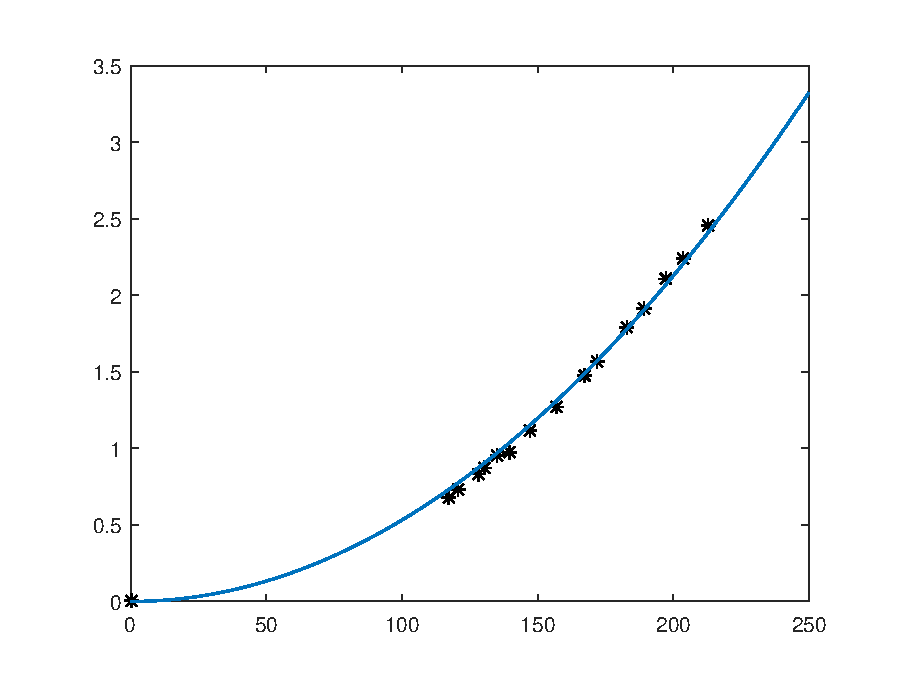
\includegraphics[scale=0.8]{figures/ThrustGraph}
%	\caption{Data from the thrust test approximated by a parabolic curve.}
%	\label{ThrustGraph}
%\end{figure}
The resulting FINISH THIS.
